\chapter{Compensador analógico} \chapterlabel{Informe/6-CompensadorAnalogico} \label{cap:Compensador Analogico}

En este capítulo se analiza la dinámica de la planta y se utilizan distintas estrategias para conseguir que el sistema presente el comportamiento deseado. Debido a la naturaleza inestable de la planta se propone una estrategia de control que logre estabilizar el sistema mediante un lazo de control interno y luego, mediante un lazo externo, mejorar su comportamiento. 


\begin{figure}[H]
	\centering
	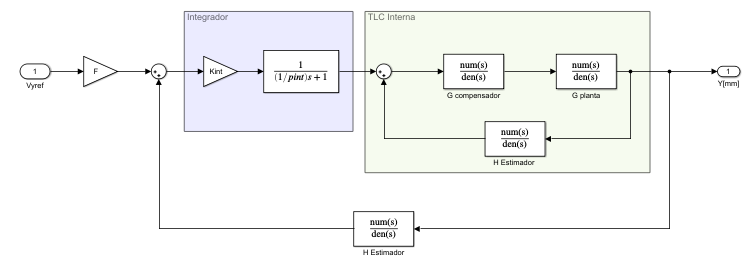
\includegraphics[scale=0.8]{Diagrama-en-bloques-comp.png}
	\caption{Diagrama simplificado del sistema completo.}
	\label{fig:diag-en-bloques-comp}
\end{figure}
\colorbox{red}{Agregar diagrama generico con: compensador interno, externo, planta  H y Gin}

\section{Lazo de realimentación interno}

En esta sección se diseña el control del lazo de realimentación interno del sistema que está compuesto por las etapas mostradas en la figura asd. 

\colorbox{red}{diagrama interno} 

Las funciones transferencias de cada bloque del diagrama asddas están dadas por:

\begin{equation*}
	G_{iL}(s) =\frac{I_L[A]}{V_{IL_{ref}}[V]}=\frac{6}{1+\frac{s}{12.17}}
\end{equation*}

\begin{equation*} 
	G_{p}(M,s)=\frac{Y_g[m]}{I_L[A]}=-\sqrt{\frac{30}{M}}*\frac{1.201}{s^{2}-4900}
\end{equation*}

\begin{equation*} 
	H_{estim}(s)=\frac{V_{estim}[V]}{Y_{g}[m]}=\frac{259.6}{(1+\frac{s}{1\:kr/s})}
\end{equation*}

A continuación se diseña el bloque del compensador interno $G_C$ para lograr la estabilidad del sistema.

\subsection{Análisis de estabilidad}

Para realizar el análisis de estabilidad se parte de las transferencias de la planta $G_{p}(s)$ para una masa de $30\:kg$, de la del controlador de corriente $G_{iL}(s)$ y de la del lazo de realimentación $H_{estim}(s)$. A partir de ellas se obtiene  la transferencia a lazo abierto total $GH_T(s)$ mostrada en la expresión \ref{eq_GT2}.

\begin{equation*} \label{eq_GT1}
	GH_T(s)=G_{p}(s)*G_{iL}(s)*H_{estim}(s) 
\end{equation*}

\begin{equation} \label{eq_GT2}
		GH_T(s)=\frac{0.38}{(1-(\frac{s}{70\:r/s})^2)(\frac{s}{12.17\:r/s }+1)(1+\frac{s}{1\:kr/s}) }	
\end{equation}

\noindent A continuación se procede a analizar la respuesta en frecuencia de $GH_T(s)$ y a diseñar un compensador adecuado. Luego, se verificará la estabilidad para una masa de $1\:kg$, que corresponde a la mínima con la que trabaja el sistema.


\noindent Con la transferencia de la ecuación  \ref{eq_GT2} se  grafica el diagrama de Bode y el de Nyquist. Estos se muestran en las figuras \ref{fig:Diag_Bode_lazo_abierto_30kg} y \ref{fig:Diag_Nyquist_lazo_abierto_30kg} respectivamente.

\begin{figure}[H]
	\centering
	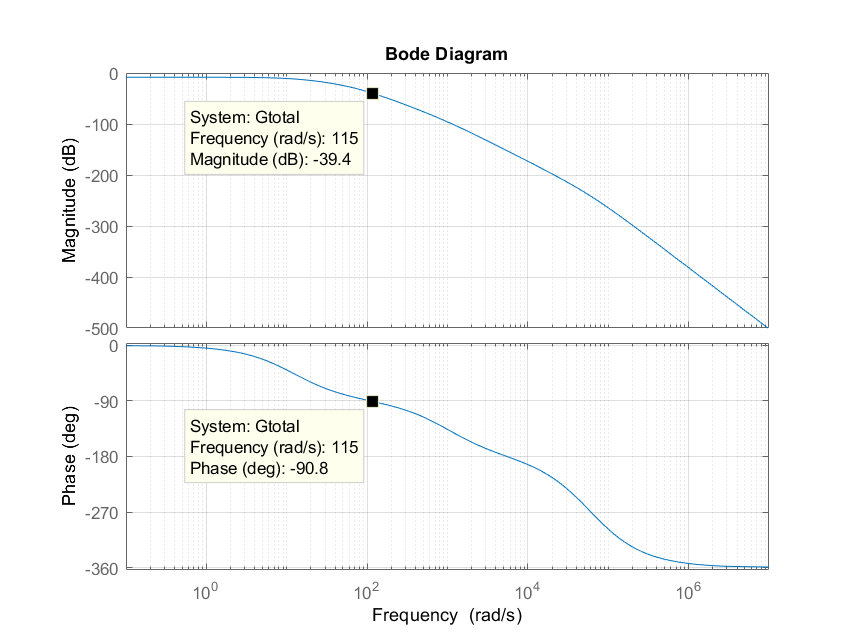
\includegraphics[scale=0.8]{bode_planta_30kg.png}
	\caption{Diagrama de Bode de lazo abierto $GH_T$ con $M=\:30 kg$.}
	\label{fig:Diag_Bode_lazo_abierto_30kg}
\end{figure}

\begin{figure}[H]
	\centering
	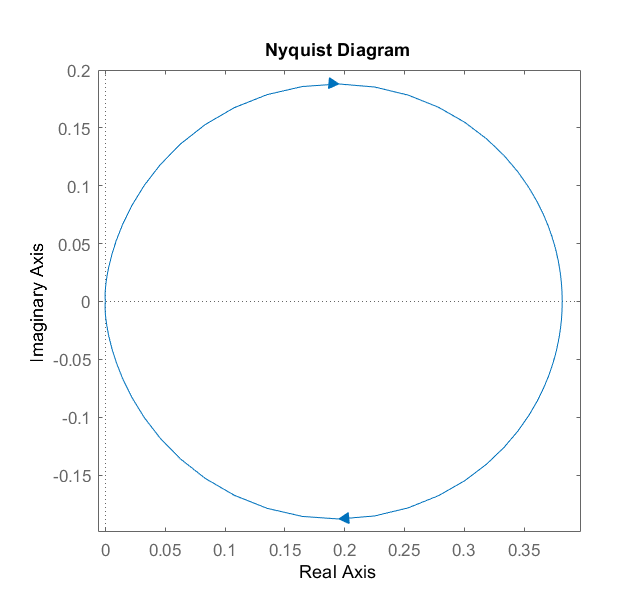
\includegraphics[scale=0.6]{nyquist_planta_30kg.png}
	\caption{Diagrama de Nyquist de $GH_T$ con $M=30\:kg$.}
	\label{fig:Diag_Nyquist_lazo_abierto_30kg}
\end{figure}


%------------------

El sistema presenta realimentación negativa. Por lo tanto, para analizar su estabilidad por medio del criterio de Nyquist, se debe determinar la cantidad de giros de $GH_T$ alrededor del punto $-1+j0$ en la figura \ref{fig:Diag_Nyquist_lazo_abierto_30kg} y la cantidad de polos en el semiplano derecho de la función transferencia $GH_T$. El sistema resultará estable si se cumple la condición 123123, donde N es la cantidad de giros, y z y p corresponden a ..

N = z -p
%----------------------------


A partir del diagrama de la figura \ref{fig:Diag_Nyquist_lazo_abierto_30kg} 

El sistema presenta realimentación negativa. Por lo tanto, para analizar su estabilidad por medio del criterio de Nyquist, se debe determinar la cantidad de giros de $GH_T$ alrededor del punto $-1+j0$ en la figura \ref{fig:Diag_Nyquist_lazo_abierto_30kg}. Es posible notar que no hay giros alrededor de este punto. Por lo tanto, considerando que $GH_{T}$ tiene un polo en el semiplano derecho es posible determinar que el sistema realimentado es inestable.

%Si L(s) es internamente estable y tiene un total de P polos inestables (en bucle abierto), el bucle cerrado ser´a estable sí y sólo sí −1 es rodeado P veces en sentido antihorario por el grafo de L(jω).


 Por lo tanto, a partir de la figura \ref{fig:Diag_Nyquist_lazo_abierto_30kg} y la ecuación \label{eq_GT2}, es posible determinar que no hay giros alrededor del punto $-1+j0$ y que existe un polo en el semiplano derecho. Por lo tanto, considerando que $GH_{T}$ tiene un polo en el semiplano derecho es posible determinar que el sistema realimentado es inestable.

 

Este analiza, para un sistema con realimentación negativa, la cantidad de giros de $1+GH_T$ alrededor del origen. Lo que es equivalente a analizar los giros de GH alrededor del punto $-1+j0$ en la figura \ref{fig:Diag_Nyquist_lazo_abierto_30kg}. 

A partir del diagrama de la figura \ref{fig:Diag_Nyquist_lazo_abierto_30kg} se puede analizar su estabilidad por medio del criterio de Nyquist. Este analiza, para un sistema con realimentación negativa, la cantidad de giros de $1+GH_T$ alrededor del origen. Lo que es equivalente a analizar los giros de GH alrededor del punto $-1+j0$ en la figura \ref{fig:Diag_Nyquist_lazo_abierto_30kg}. 

Es posible notar que no hay giros alrededor de -1. Por lo tanto, considerando que $GH_{T}$ tiene un polo en el semiplano derecho es posible determinar que el sistema realimentado es inestable.

Para lograr estabilizar este sistema se debe utilizar realimentación positiva en el diagrama en bloques, de manera que ahora se deben observar los giros de $1-GH_T$ alrededor del origen, que equivale a observar $GH_T$ alrededor del punto $+1+j0$. Además, se debe generar una zona en el diagrama de Nyquist donde exista un giro alrededor de 1 en sentido antihorario. Para ello, es necesario aumentar la fase para que pueda superar el valor de 0$\mathrm{{}^\circ}$.  Para que esto se cumpla, el diagrama de Nyquist debe tener una forma como la  mostrada en la figura \ref{fig:nyquist-deseado-analog}.

A partir del diagrama de Nyquist de la figura \ref{fig:Diag_Nyquist_lazo_abierto_30kg} es posible notar que no hay giros alrededor de -1. Por lo tanto, considerando que $GH_{T}$ tiene un polo en el semiplano derecho es posible determinar que el sistema realimentado es inestable.

\colorbox{red}{Corregir esto}

De esta forma, para lograr la estabilidad se debe realimentar positivamente y generar una zona en el diagrama de Nyquist donde exista un giro alrededor de -1 en sentido antihorario. Sin embargo, debido a que ahora se utiliza realimentación positiva, el diagrama de Nyquist debe analizarse en torno al 1 positivo. Para generar el giro en sentido antihorario es necesario aumentar la fase para que pueda superar el valor de 0$\mathrm{{}^\circ}$.  Para que esto se cumpla, el diagrama de Nyquist debe tener una forma como la  mostrada en la figura \ref{fig:nyquist-deseado-analog}.

\begin{figure}[H]
	\centering
	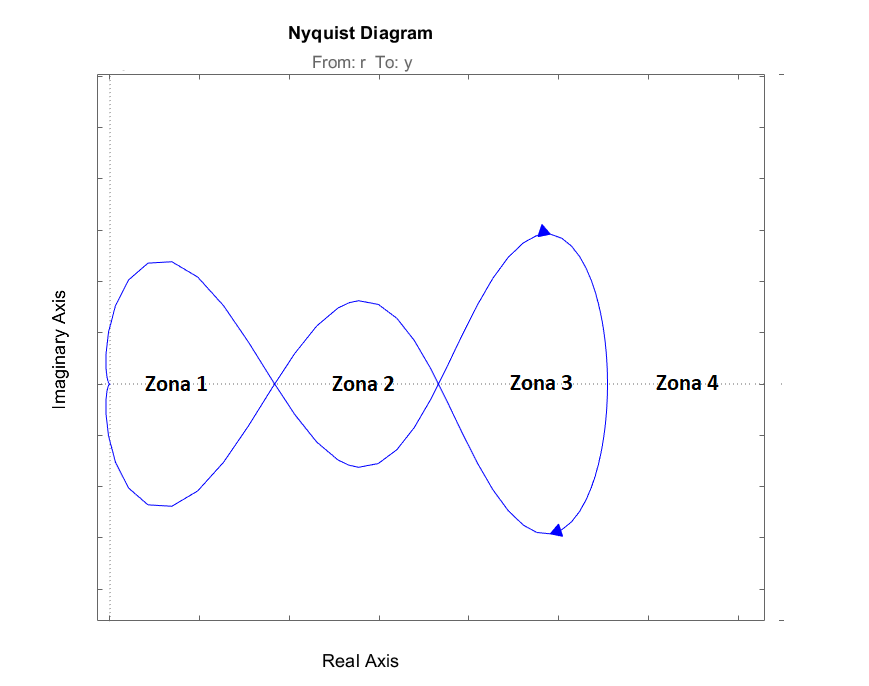
\includegraphics[scale=0.6]{Nyquist-deseado-analog.png}
	\caption{Forma del diagrama de Nyquist deseado.}
	\label{fig:nyquist-deseado-analog}
\end{figure}

\subsection{Diseño de la red de adelanto de fase}
Para lograr el comportamiento del sistema como en la figura 	\ref{fig:nyquist-deseado-analog} se debe tener en cuenta que el m\'{o}dulo de la transferencia de lazo abierto en el primer cruce de la fase por 0$\mathrm{{}^\circ}$ debe ser mayor a $0\:dB$ y, en el segundo cruce, menor. De esta forma, al observar la figura \ref{fig:Diag_Bode_lazo_abierto_30kg} se decide adelantar la fase 100º en aproximadamente $200\:r/s$. Esto se logra mediante el uso de dos redes de adelanto de fase de 65$\mathrm{{}^\circ}$ cada una.


\noindent De esta forma, las ecuaciones de dise\~{n}o resultan:

\begin{equation*}
	\begin{aligned}
		&W_0 =200\:r/s\\
		&{\varphi }_{max} =65\textrm{º}\\
		&\alpha =\frac{1+sen({\varphi }_{max})}{1-sen{(\varphi }_{max})}=20.346491\\
		&W_c =\frac{W_0}{\sqrt{\alpha }}=\ 44.3\:r/s\\
		&W_p =\sqrt{\alpha }*W_0=902.1\: r/s\\
	\end{aligned}
\end{equation*} 
\noindent Finalmente, se llega a la transferencia del controlador:

\begin{equation}  
	G_c(s)=K*{[20.346*\frac{(s+44.3)}{(s+902.1)}]}^2
\end{equation} 

\noindent En la figura \ref{fig:bode-analog-compensado-para-k-1} se muestra el diagrama de bode de ${GH}_T*G_C$ con $K=1$. Se puede observar que la ganancia $K$ puede adoptar valores desde $15.7\:dB$ hasta $35.5\:dB$ aproximadamente. Al considerar que el sistema debe soportar una masa variable entre $1\:kg$ y $30\:kg$, y que la ganancia de la transferencia de la planta para $1\:kg$ es de $5.5$ veces ($14\:dB$) mayor que para $30\:kg$, se debe adoptar una ganancia del compensador que mantenga la estabilidad para estos dos casos. Es decir, la ganancia m\'{i}nima es de $15.7\:dB$ y la m\'{a}xima es de $35.5\:dB - 14\:dB = 21.5\:dB$. Por lo tanto, se elige que el cruce por cero de la ganancia se encuentre ahora en $88\:r/s$, lo que significa que $K=20\:dB\ \equiv \ 10\: veces$.


\begin{figure}[H]
	\centering
	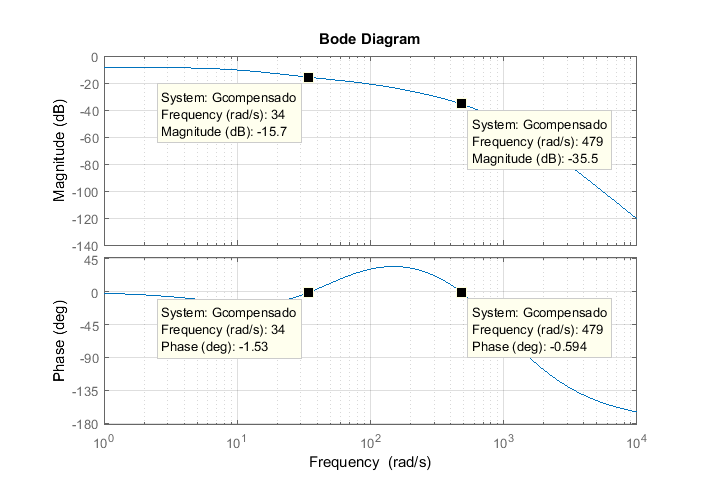
\includegraphics[scale=0.85]{Bode-k-1-M-30.png}
	\caption{Diagrama de Bode de $GH_T*G_C$ para $K=1$ y $M=30\:kg$.}
	\label{fig:bode-analog-compensado-para-k-1}
\end{figure}

\noindent En la figura \ref{fig:bode-analog-compensado-para-k-10} se muestra el diagrama de Bode al considerar la ganancia del compensador. En ella se puede observar que se  cumple con el criterio de estabilidad, puesto que en el primer cruce por 0º, la magnitud es mayor a 0 dB y en el segundo cruce, menor. Adem\'{a}s, en la figura \ref{fig:nyquist-analog-para-k-10} se puede ver que la forma del diagrama de Nyquist es como la deseada.

\begin{figure}[H]
	\centering
	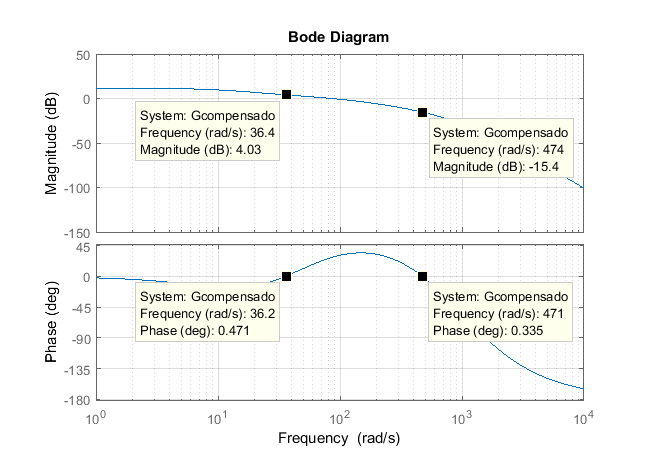
\includegraphics[scale=0.8]{Bode-k-10-M-30.png}
	\caption{Diagrama de Bode de $GH_{T}*G_C$ para $K=10$ y $M=30\:kg$.}
	\label{fig:bode-analog-compensado-para-k-10}
\end{figure}

\begin{figure}[H]
	\centering
	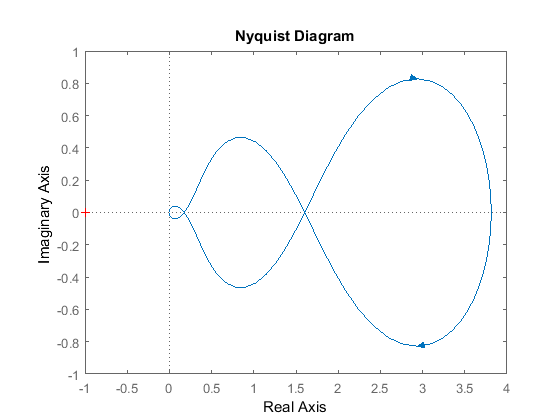
\includegraphics[scale=0.8]{Nyquist-k-10-M-30.png}
	\caption{Diagrama de Nyquist de $GH_T*G_C$ para $K=\:10$ y $M=30\:kg$.}
	\label{fig:nyquist-analog-para-k-10}
\end{figure}

\subsection{Transferencia de lazo cerrado}

Finalmente se puede expresar la función transferencia de lazo cerrado del lazo de control interno como:
%
%-3.6301e05 (s+1000) (s+44.3)^2
%------------------------------------------------------------------
%(s+304.3) (s+115.6) (s^2 + 44.84s + 2588) (s^2 + 2352s + 1.498e06)


\begin{equation}
	TLC_{interna}(s)=\frac{Y_g}{V_{ref_c}}=\frac{G_c*G_{p}*G_{iL}}{1-G_c*G_{p}*G_{iL}*H_{estim}}
	%	\frac{-3.6301*}{den}
\end{equation}

Por último se simuló la respuesta del sistema a un escalón de amplitud unitaria en la señal $V_{ref_c}$. La salida es un valor de distancia de entrehierro $Y_g$ en metros. En la figura \ref{fig:rta-escalon-k-10-m-30} se puede observar la respuesta al escalón del sistema con masa de $30\:kg$.

\colorbox{red}{Ver como acomodar lo de la respuesta al escalon (y para 1kg tambien)}

\begin{figure}[H]
	\centering
	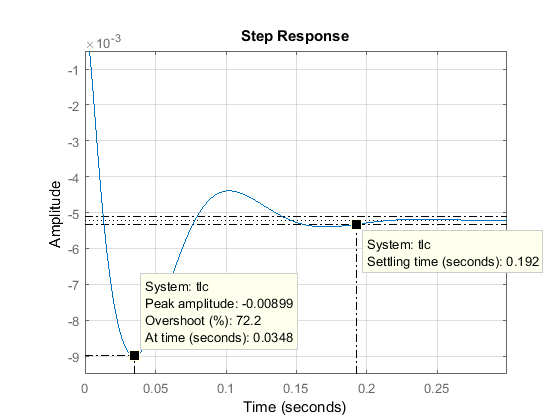
\includegraphics[scale=0.80]{Respuesta-al-escalon-K-10-M-30Kg.png}
	\caption{Respuesta al escalón para $M=30\:kg$.}
	\label{fig:rta-escalon-k-10-m-30}
\end{figure}

\subsection{Verificación de estabilidad con masa de 1 kg}

\noindent Se verifica la estabilidad del sistema  para el caso en que la masa sea de $1\:kg$ con el compensador dise\~{n}ado para el caso de masa m\'{a}xima. Para ello, se analizan los diagramas de Bode y Nyquist mostrados en las figuras \ref{fig:bode-analog-para-M-1Kg} y \ref{fig:nyquist-analog-para-M-1Kg}. Adem\'{a}s, en la figura \ref{fig:respuesta-analog-al-escalon-para-M-1Kg} puede observarse la respuesta al escal\'{o}n. A partir de ellos, es posible verificar que el sistema resulta estable para todo el rango de masas en el que opera el sistema. 


\begin{figure}[H]
	\centering
	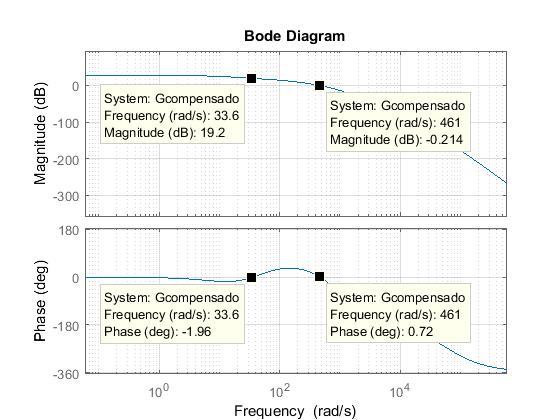
\includegraphics[scale=0.80]{bodecompensado1kg.png}
	\caption{Diagrama de Bode de $GH_T*G_c$ para $M=1\:kg$.}
	\label{fig:bode-analog-para-M-1Kg}
\end{figure}

\begin{figure}[H]
	\centering
	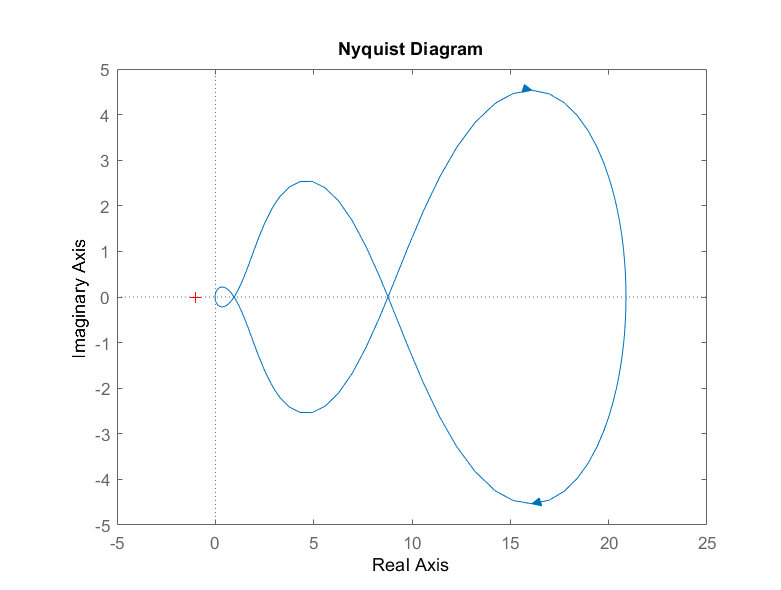
\includegraphics[scale=0.55]{nyquistcompensado1kg.png}
	\caption{Diagrama de Nyquist de $GH_T*G_C$ para $M=1\:kg$.}
	\label{fig:nyquist-analog-para-M-1Kg}
\end{figure}

\begin{figure}[H]
	\centering
	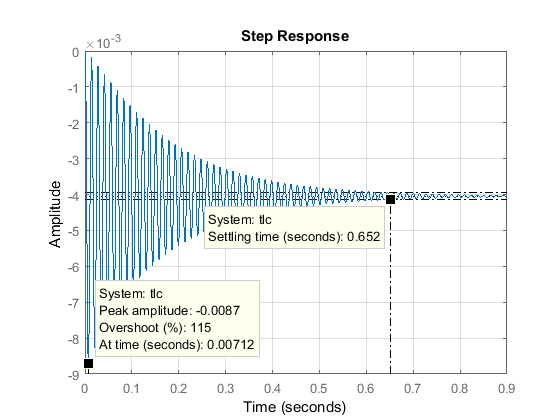
\includegraphics[scale=0.80]{rtaescaloncompensado1kg.png}
	\caption{Respuesta al escalón para $M=1\:kg$.}
	\label{fig:respuesta-analog-al-escalon-para-M-1Kg}
\end{figure}

\subsection{Implementación circuital de la red de adelanto de fase}

\noindent Para cada etapa del compensador por adelanto se utiliza la topología mostrada en la figura \ref{fig:red-adelanto-fase}. Consiste en  un polo y un cero con ganancia unitaria (si Ra = Rb). Luego, se agrega la ganancia como una etapa separada.

\begin{figure}[H]
	\centering
	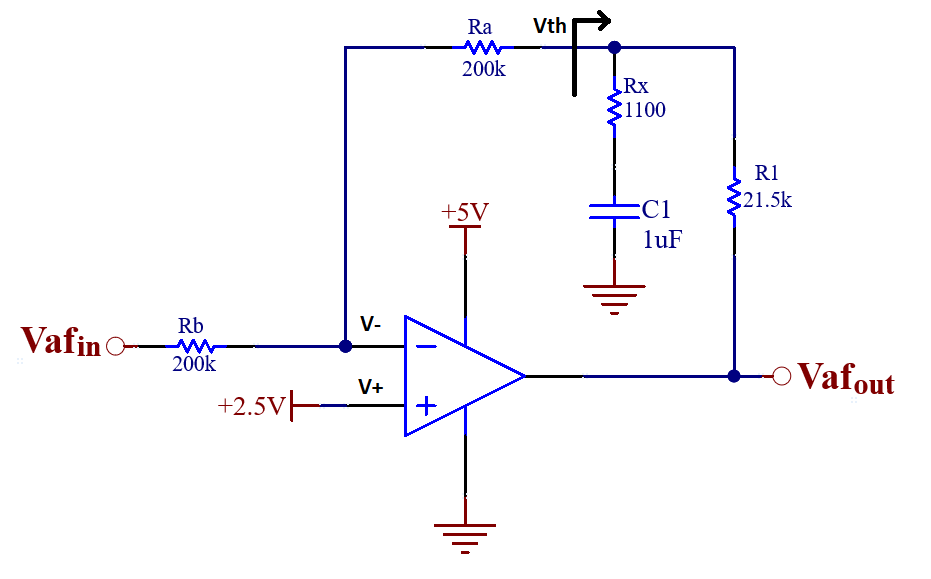
\includegraphics[scale=0.55]{Red-adelanto-fase.png}
	\caption{Diseño circuital de una red de adelanto de fase.}
	\label{fig:red-adelanto-fase}
\end{figure}

\noindent La transferencia de lazo cerrado de esta etapa es:

\begin{equation} 
	\frac{V_{out}}{V_{in}}= - \frac{R_a}{R_b}*\frac{1+sC(R_x+R_1)}{1+sCR_x}
\end{equation}

\noindent Por lo tanto, para tener un polo en $902.1\:Hz$ y un cero en $44.3\:Hz$, al elegir un capacitor $C = 1\:uF$, resulta en $R_x = 1100\:\Omega$ y $R_1 = 21.5\:k\Omega$. Además, se elige $R_a = R_b = 200\:k\Omega$ para obtener una ganancia unitaria. Luego, la ganancia del compensador se obtiene con una etapa amplificadora.
Para ello, se utiliza el circuito mostrado en la figura \ref{fig:ganancia-compensador}. Para lograr una ganancia de $K=10$ se utiliza $R_{322} = 1\:k\Omega$ y $R_{323} = 10\:k\Omega$.


\begin{figure}[H]
	\centering
	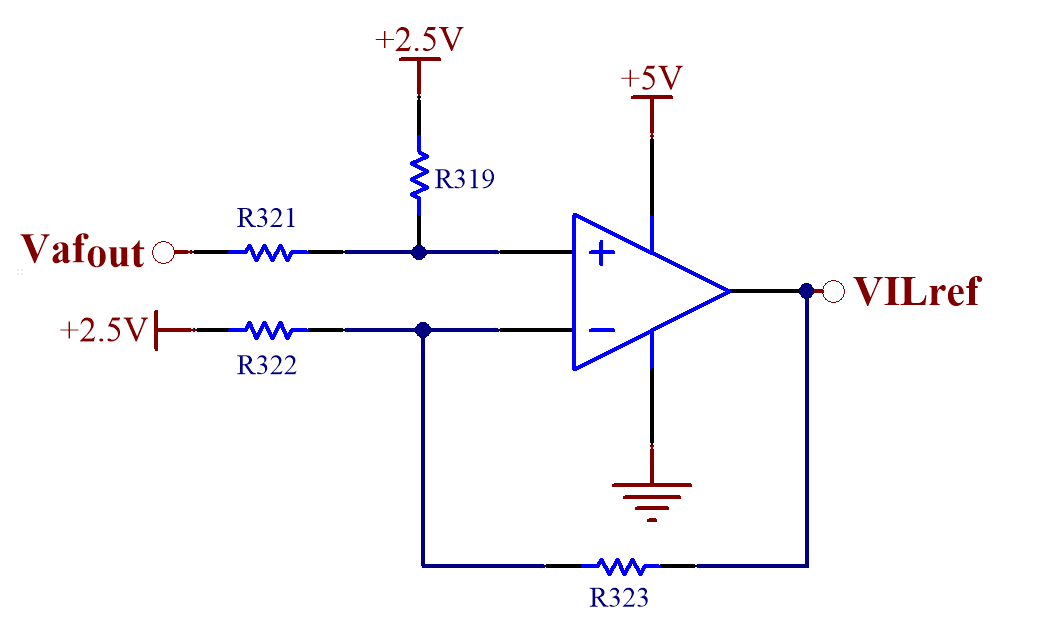
\includegraphics[scale=0.6]{Ganancia-compensador.png}
	\caption{Etapa de ganancia del compensador.}
	\label{fig:ganancia-compensador}
\end{figure}

\section{Lazo del realimentación externo}
\subsection{Diseño del integrador}

\noindent Se plantea un lazo de realimentaci\'{o}n externo como se muestra en la  figura \ref{fig:diag-en-bloques-comp}. En el lazo de realimentaci\'{o}n interno act\'{u}a el compensador por adelanto de fase dise\~{n}ado previamente y, en el externo, un controlador del tipo integral. De esta forma, se logra suavizar la respuesta al escal\'{o}n del sistema y eliminar el error en r\'{e}gimen permanente.


\noindent Para el an\'{a}lisis se considera como realimentaci\'{o}n: 

\[H_{estim}=\frac{V_{estim}}{Y[m]}= - \frac{259.6}{(1 + \frac{s}{1\:k})*(1+\frac{s}{60\:k})^2}\] 

\noindent La cadena de avance con masa de $30\:kg$ es:

\[G[m=30]=TLC_{interna}(s)[m=30]*G_{integ}\] 

\noindent Se  plantea un compensador del tipo :

\[G_{integ}\ =\ k_{int}\ *\ \frac{1}{(1+(\frac{s}{p_{int}}))}\]

\noindent Debido a que un integrador con polo en el origen tiene una ganancia infinita en contínua, no sería adecuado implementarlo de esta manera en el circuito. Por lo tanto, se ubica el polo en $0.1\:rad/s$ de forma tal que permita limitar dicha ganancia y ser de carácter integrativo para las frecuencias de la planta. Sin embargo, esta modificación provoca que la cancelación del error en régimen permanente no sea completa.
%, pero de todas maneras sea pequeña en comparación con la distancia de separación.

%Debido a que no usamos un integrador ideal, la respuesta al escalón presentará un cierto error.

Inicialmente se analiza la estabilidad del sistema con $K_{int} = 1$ por medio del lugar de raíces mostrado en la figura \ref{fig:lugar-de-raices-con-integrador-analog}.

\noindent Para este lazo de realimentación externo también debe utilizarse realimentación positiva, puesto que la TLC interna del sistema presenta una ganancia negativa.


\begin{figure}[H]
	\centering
	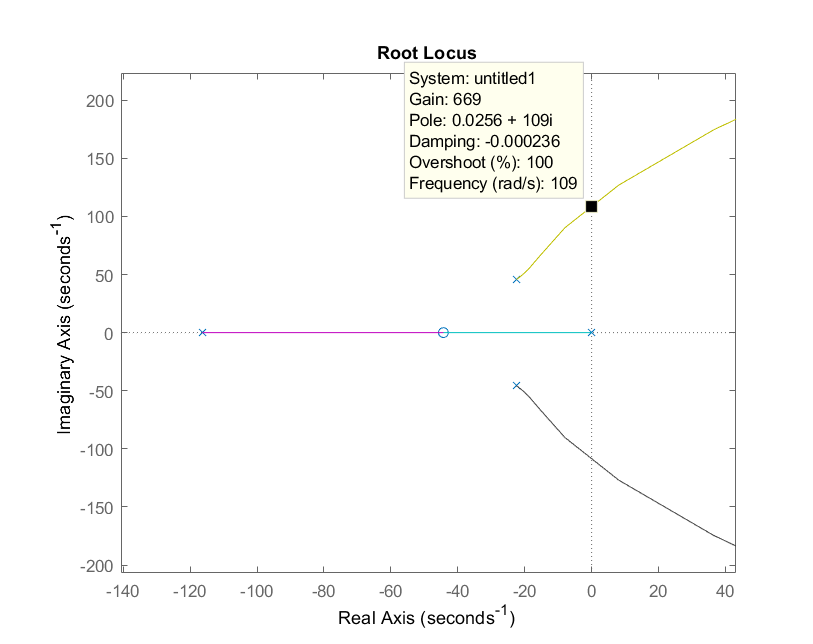
\includegraphics[scale=0.5]{rlocusconintegrador30kg.png}
	\caption{Lugar de raíces con el integrador.}
	\label{fig:lugar-de-raices-con-integrador-analog}
\end{figure}

\noindent En la figura \ref{fig:lugar-de-raices-con-integrador-analog} se puede observar que, para que se mantenga la estabilidad del sistema, la ganancia del integrador ($K_{int}$) debe ser menor a 669. Teniendo esto en cuenta, en la figura \ref{fig:respuesta-al-escalon-con-k-1-M-30-analog} se muestra la respuesta al escal\'{o}n del sistema compensado con el integrador para una ganancia de $K_{int}=1$.  Es posible observar que, si bien no presenta oscilaciones, el tiempo de establecimiento es de aproximadamente $16.6 \:s$. Por lo tanto, se decide aumentar el valor de ganancia hasta obtener una relaci\'{o}n aceptable entre el tiempo de respuesta y el sobrepico.

\begin{figure}[H]
	\centering
	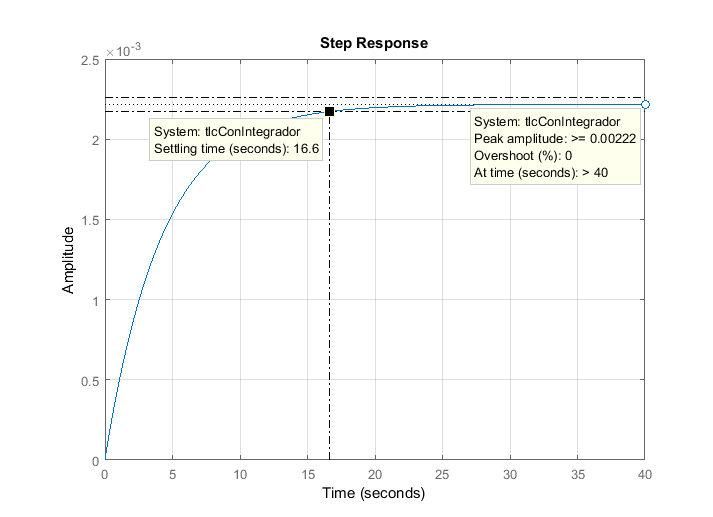
\includegraphics[scale=0.85]{stepresponseintegradorkint_1_m_30.png}
	\caption{Respuesta al escalón con integrador con $K_{int} =1$ y $M=30\:kg$.}
	\label{fig:respuesta-al-escalon-con-k-1-M-30-analog}
\end{figure}

\noindent En la figura \ref{fig:respuesta-al-escalon-con-k-50-M-30}, se observa la respuesta al escal\'{o}n para una ganancia del integrador de $K_{int}=50$ que resulta en un tiempo de establecimiento de $0.6\:s$ y un \textsl{overshoot} de 0\%. Por lo tanto, se adopta este valor de ganancia para el dise\~{n}o del integrador.

\begin{figure}[H]
	\centering
	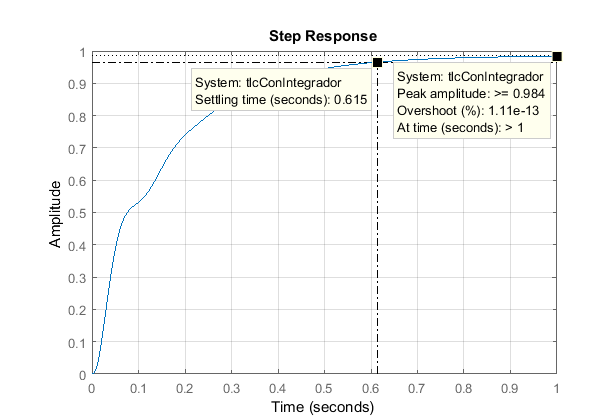
\includegraphics[scale=0.85]{stepresponseintegradorkint_50_m_30.png}
	\caption{Respuesta al escalón con integrador para $K_{int}=50$ y $M = 30\:kg$.}
	\label{fig:respuesta-al-escalon-con-k-50-M-30}
\end{figure}

\noindent La respuesta al escal\'{o}n cuando la masa es de $1 \:kg$ se muestra en la figura \ref{fig:respuesta-al-escalon-con-k-50-M-1}. All\'{i} se puede observar que el tiempo de establecimiento es de $0.74\:s$ y que no presenta sobrepicos.

\begin{figure}[H]
	\centering
	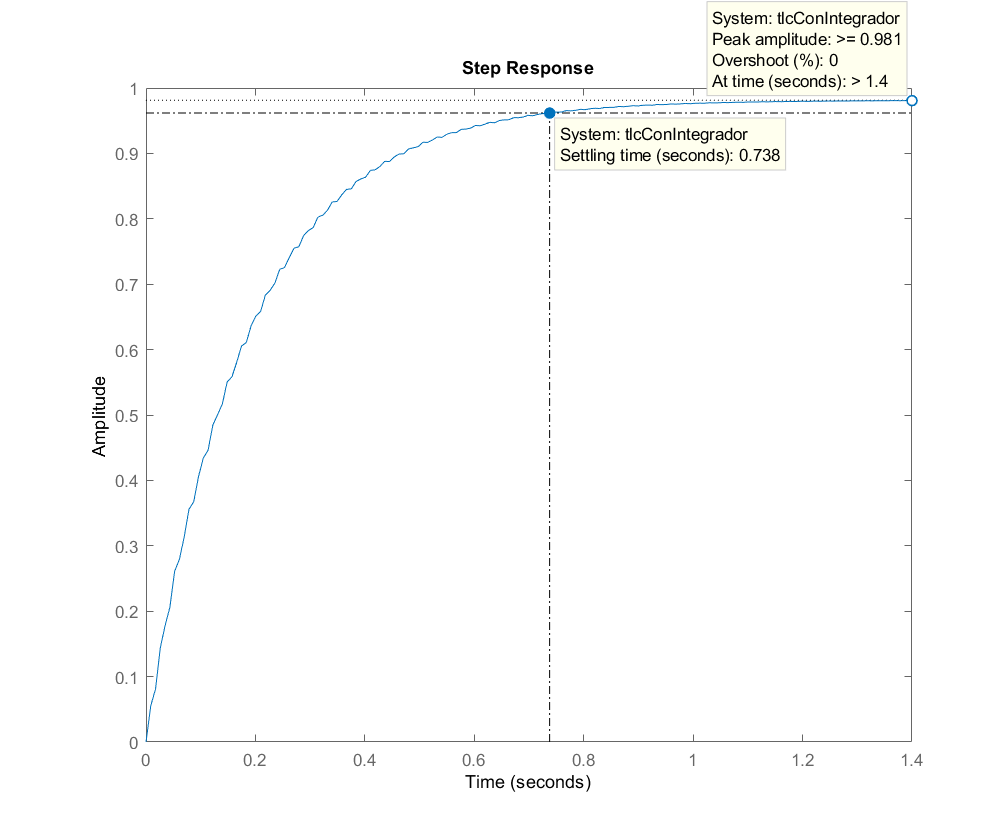
\includegraphics[scale=0.85]{stepresponseintegradorkint_50_m_1.png}
	\caption{Respuesta al escalón con integrador para $K_{int} =50$ y $M = 1 \:kg$.}
	\label{fig:respuesta-al-escalon-con-k-50-M-1}
\end{figure}



\subsection{Implementación circuital del integrador}

\noindent En la figura \ref{fig:circuito-integrador} se puede observar la topología y los valores utilizados en cada componente para el diseño del circuito integrador. 

\begin{figure}[H]
	\centering
	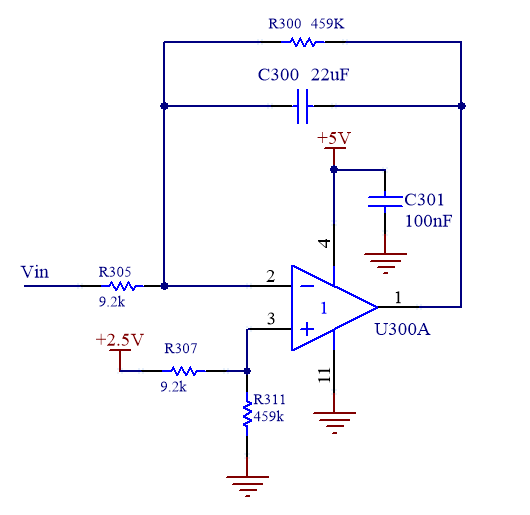
\includegraphics[scale=0.6]{Circuito-integrador.png}
	\caption{Implementación circuital del integrador.}
	\label{fig:circuito-integrador}
	\end{figure}
\section{Etapa de entrada}
\subsection{Cálculo de ganancia de entrada}

\noindent La ganancia de la TLC correspondiente a la ganancia de contínua total de los bloques con el integrador ya incorporado, resulta:

\begin{equation} 
	G_{TLC_{final}} \simeq \frac{1}{H_{estim}} = - \frac{1}{259.6}
\end{equation}

\begin{figure}[H]
	\centering
	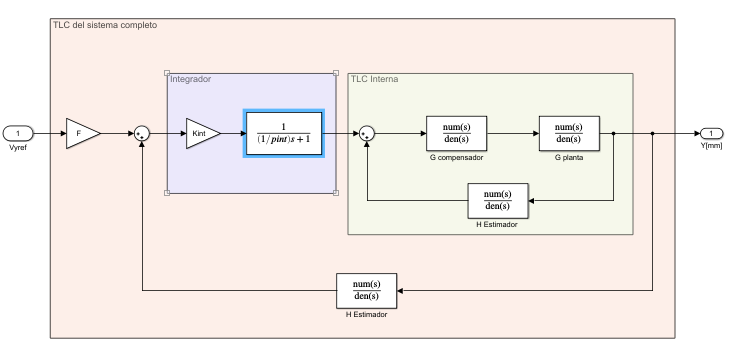
\includegraphics[scale=0.8]{Diagrama-en-bloques-compensador.png}
	\caption{Diagrama en bloques final.}
	\label{fig:diag-bloques-compensador}
\end{figure}

\noindent Por lo tanto, con $F=-1$ y los rangos de posición de $2\:mm$ a $5\:mm$ como mínimo y máximo respectivamente se llega a lo siguiente:

\begin{equation} 
	Y_g[m] = F * (-\frac{1}{259.6})*V_{in} =\frac{1}{259.6}*V_{in} 
\end{equation}

\noindent La realimentación tiene un \textsl{set-point} de $3.4\:V$. Por lo tanto, se le suma a $V_{in}$ el mismo valor.

\noindent Los valores finales son:


\begin{table}[H]
	\begin{center}
		\begin{tabular}{| c | c |}
			\hline
			$Y_g\:[mm]$ & $V_{in}[V]$\\ \hline
			5 & 4.7\\ \hline
			4 & 4.44 \\ \hline
			3 & 4.18\\ \hline
			2 &	3.92 \\ \hline		
		\end{tabular}
		\caption{Tensión de referencia $[V_{in}]$ Vs separación deseada [$Y_g$].}
		\label{tension-ref-vs-separacion-deseada}
	\end{center}
\end{table}

\subsection{Implementación circuital}

\noindent Para poder modificar la distancia de separación se ingresa al sistema con una tensión variable, la cual corresponde a una posición de referencia. Para ello se utiliza el circuito mostrado en la figura \ref{fig:etapa-de-entrada}.

\begin{figure}[H]
	\centering
	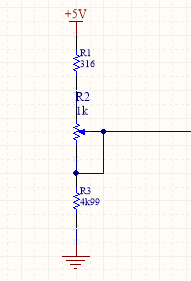
\includegraphics[scale=0.8]{Etapa-de-entrada.png}
	\caption{ Etapa de entrada.}
	\label{fig:etapa-de-entrada}
\end{figure}

 
 \noindent Se utiliza una resistencia variable de $1\:k\Omega$ y dos con valores fijos. Para poder excursionar la tensión de referencia entre $3.92\:V$ y $4.7\:V$, los valores de las resistencias $R_1$ y $R_3$ deben ser de $4911\:\Omega$ y $313.5\:\Omega$ respectivamente. 
 
\noindent Por lo tanto, al adoptar un valor comercial para ellas, resulta en $R_1 = 316 \:\Omega$ y en $R_3 = 4990 \:\Omega$.
 
\noindent De esta forma, el valor de tensión máximo para la referencia de posición queda en $4.69\:V$ y el mínimo en $3.96\:V$.
 
